\chapter*{Math Challenge}

\section*{Arithmetic}

i). Find the value of the product of fractions: $$\left(\frac{60}{21}\right)\times\left(\frac{1}{33}\right)\times\left(\frac{6}{5}\right)\times \left(\frac{35}{8}\right)$$\\

%Sug: 1. ¿Cómo se multiplican las fracciones?. 2. Factoriza y cancela (no se tiene que hacer ninguna multiplicación). Recuerda que el orden de los factores no altera el producto (tanto el de arriba como el de abajo). \\

ii). What is the value of $$\left(\frac{1}{2}\right)\times\left(\frac{2}{3}\right)\times\left(\frac{3}{4}\right)\times\cdots \times\left(\frac{998}{999}\right)\times\left( \frac{999}{1000}\right)?$$

iii). Add the first thirty three natural numbers $$1+2+3+4+5+\cdots+31+32 +33.$$

iv). Compute the sum $$1+2+3+4+\cdots +1998+1999+2000.$$

%Sug: El problema v) es más sencillo. Inténtalo primero. 1A. Suma dos veces (al derecho y al revés). 1B. Arreglo triangular de puntos. \\

v). Compute the sum of the first thousand odd numbers: $$1+3+5+7+\cdots +1995+1997+1999.$$

%Sug: A. Arreglo cuadrangular de puntos, o B. Suma dos veces (al derecho y al revés). \\

vi). Compute the sum $$1+2+2^2+2^3+\cdots +2^{18}+2^{19}.$$

%Sug: 1. Haz una conjetura directa revisando casos pequeños: 1, 1+2, 1+2+4, 1+2+4+8, \dots 2. ¿Cómo se ven esos números en base binaria?. \\

vii). Now with powers of three: $$1+3+3^2+3^3+\cdots +3^{18}+3^{19}$$

%Sug: 1. Usa base tres. 2. Multiplica por dos y suma uno. \\

viii). Try to compute the sum of cubes: $$1^3+2^3+3^3+4^3+\cdots +98^3+99^3+100^3$$

%Sug: Haz una conjetura directa revisando casos pequeños. \\

ix). Now try with squares: $$1^2+2^2+3^2+4^2+\cdots +98^2+99^2+100^2.$$

%Sug: Aquí no es nada fácil obtener una conjetura directa (cough!, cough!, $\frac{1}{6}n(n+1)(2n+1)$).\\

x). Find the value of $$1\times2+2\times3+3\times4+\cdots +99\times100+100\times101.$$

%Sug: Suma los ejercicios v) y ix).\\

%Notas al Instructor: i) y ii). Revisar manejo de operaciones de fracciones. iii)-v). Preguntar cómo llegaron al resultado. No anticipar truco de sumar dos veces al derecho y al revés. vi) y vii). Revisar manejo de bases numéricas.  viii)-x). Invitación a la inducción matemática: ¿Cuánto vale la diferencia de términos consecutivos de tu fórmula?. Repaso de manejo de sumas y multiplicaciones de fracciones con variables. \\

\vspace{.5cm}
\begin{flushright}
Questions/Hints/Solutions: 

ei.turbomath@gmail.com

473-740-9385
\end{flushright}

\newpage

\section*{Chessboard tiling problems}

\begin{multicols}{2}
i). You are given ten tetris blocks, two of each type (Fig. 1). Decide:

Is it possible to build a rectangle using all ten blocks, without holes and without overlaps?\\

%Sug: Intenta con un rectángulo de 8\times 5. \\

ii). If you now have three blocks of each type: Is it possible, or not?\\

%Sug: Mejor piénsale primero al iii) y al iv). \\

iii). Two opposite corners of a chessboard are removed (Fig. 2).  

Is it possible to cover the rest with $31$ domino tiles of size $2\times 1$?\\

%Sug: ¿De qué colores son las esquinas? Intenta primero con tableros más pequeños. \\

iv). Consider a $5\times 5$ grid with three corners removed, as in Figure 3.
  
Is it possible to cover the rest with $11$ dominoes?\\

%Sug: ¿De qué colores son las esquinas?

v). A $7\times 7$ board may be covered using $16$ tiles of size $3\times 1$ and a single square tile of size $1\times 1$.

Indicate in figure 4 all possible locations of the $1\times 1$ square.

%Sug: No se pueden todas. Colorear con tres colores por diagonales para descartar algunas posiciones.

\columnbreak

\begin{tikzpicture}[line cap=round,line join=round,>=triangle 45,x=.5cm,y=.5cm]
\draw [line width=1pt] (0,0)-- (2,0);
\draw [line width=1pt] (0,0)-- (0,2);
\draw [line width=1pt] (0,2)-- (2,2);
\draw [line width=1pt] (2,2)-- (2,0);
\draw [line width=1pt] (0,1)-- (2,1);
\draw [line width=1pt] (1,2)-- (1,0);
\draw [line width=1pt] (5.6,2.6)-- (7.6,2.6);
\draw [line width=1pt] (7.6,2.6)-- (7.6,0.6);
\draw [line width=1pt] (6.6,0.6)-- (8.6,0.6);
\draw [line width=1pt] (8.6,0.6)-- (8.6,1.6);
\draw [line width=1pt] (8.6,1.6)-- (5.6,1.6);
\draw [line width=1pt] (5.6,2.6)-- (5.6,1.6);
\draw [line width=1pt] (6.6,2.6)-- (6.6,0.6);
\draw [line width=1pt] (0,4)-- (0,7);
\draw [line width=1pt] (0,7)-- (1,7);
\draw [line width=1pt] (1,7)-- (1,4);
\draw [line width=1pt] (1,4)-- (0,4);
\draw [line width=1pt] (0,5)-- (1,5);
\draw [line width=1pt] (1,6)-- (0,6);
\draw [line width=1pt] (4.5,1.2)-- (4.5,4.2);
\draw [line width=1pt] (3.5,4.2)-- (3.5,1.2);
\draw [line width=1pt] (2.5,3.2)-- (4.5,3.2);
\draw [line width=1pt] (2.5,2.2)-- (4.5,2.2);
\draw [line width=1pt] (2.5,3.2)-- (2.5,2.2);
\draw [line width=1pt] (3.5,4.2)-- (4.5,4.2);
\draw [line width=1pt] (3.5,1.2)-- (4.5,1.2);
\draw [line width=1pt] (2,7)-- (2,5);
\draw [line width=1pt] (3,5)-- (3,7);
\draw [line width=1pt] (2,7)-- (5,7);
\draw [line width=1pt] (5,6)-- (2,6);
\draw [line width=1pt] (2,5)-- (3,5);
\draw [line width=1pt] (4,7)-- (4,6);
\draw [line width=1pt] (5,7)-- (5,6);
\draw [line width=1pt] (0,4)-- (0,3);
\draw [line width=1pt] (0,3)-- (1,3);
\draw [line width=1pt] (1,3)-- (1,4);
\end{tikzpicture}

Fig. 1: Five Tetraminos,

types <<straight>>, <<L>>,  

<<square>>, <<T>> and <<Z>> \\

    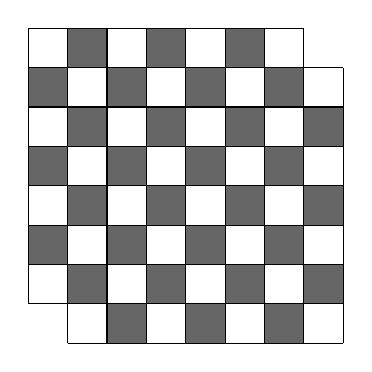
\begin{tikzpicture}[x=0.5cm,y=0.5cm]
  \foreach \i in {0,...,3} 
    \foreach \j in {0,...,3}
    \fill[line width=1pt,color=black,fill=black,fill opacity=0.6] (2*\i,2*\j) -- (2*\i,2*\j+1) -- (2*\i+1,2*\j+1) -- (2*\i+1,2*\j) -- cycle;
  \foreach \i in {0,...,3} 
    \foreach \j in {0,...,3}
        \fill[line width=1pt,color=black,fill=black,fill opacity=0.6] (2*\i+1,2*\j+1) -- (2*\i+1,2*\j+2) -- (2*\i+2,2*\j+2) -- (2*\i+2,2*\j+1) -- cycle;
        \fill[line width=1pt,color=white,fill=white,fill opacity=1] (0,0) -- (0,1) -- (1,1) -- (1,0) -- cycle;
        \fill[line width=1pt,color=white,fill=white,fill opacity=1] (7,7) -- (7,8) -- (8,8) -- (8,7) -- cycle;
    \foreach \i in {1,...,7} \draw[black] (0,\i) -- (8,\i);
    \foreach \i in {1,...,7} \draw[black] (\i,0) -- (\i,8);       
    \draw[black] (1,0) -- (8,0);
    \draw[black] (0,1) -- (0,8);
    \draw[black] (0,8) -- (7,8);
    \draw[black] (8,0) -- (8,7);
  \end{tikzpicture}

Fig. 2

 \end{multicols}
    
 Fig. 3 \hspace{.5cm}
  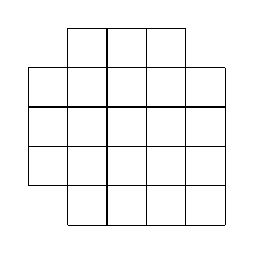
\begin{tikzpicture}[x=0.5cm,y=0.5cm]
     \foreach \i in {1,...,4} \draw[black] (0,\i) -- (5,\i);
    \foreach \i in {1,...,4} \draw[black] (\i,0) -- (\i,5);       
    \draw[black] (1,0) -- (5,0);
    \draw[black] (0,1) -- (0,4);
    \draw[black] (1,5) -- (4,5);
    \draw[black] (5,0) -- (5,4);
  \end{tikzpicture}
  \hspace{3cm} Fig. 4 \hspace{.5cm}  
  
\begin{tikzpicture}[x=0.5cm,y=0.5cm]
     \foreach \i in {0,...,7} \draw[black] (0,\i) -- (7,\i);
    \foreach \i in {0,...,7} \draw[black] (\i,0) -- (\i,7);       
  \end{tikzpicture}
  \\
   
  vi). Consider a $(2n)\times (2n)$ chessboard, without its four corners, as in Fig. 5.

For which values of $n=2,3,4,5,\dots $ is it possible to cover the rest of the board, using only <<$L$>>-shaped tetris blocks?

%Sug: i) Algunos se pueden y algunos no se pueden. ii) Para descartar n=2k, colorear con franjas negras y blancas. iii) ¿Es posible cubrir $n=b$ casillas con un número impar de tetraminos <<L>>?
Fig. 5\hspace{.5cm}
  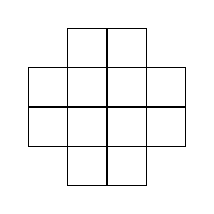
\begin{tikzpicture}[x=0.5cm,y=0.5cm]
     \foreach \i in {1,...,3} \draw[black] (0,\i) -- (4,\i);
    \foreach \i in {1,...,3} \draw[black] (\i,0) -- (\i,4);       
    \draw[black] (1,0) -- (3,0);
    \draw[black] (0,1) -- (0,3);
    \draw[black] (1,4) -- (3,4);
    \draw[black] (4,1) -- (4,3);
  \end{tikzpicture}
  $n=2$
  \hspace{.5cm}  
    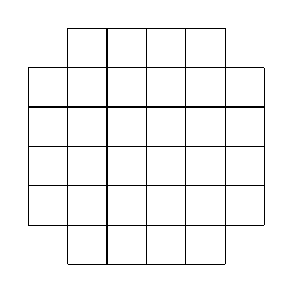
\begin{tikzpicture}[x=0.5cm,y=0.5cm]
     \foreach \i in {1,...,5} \draw[black] (0,\i) -- (6,\i);
    \foreach \i in {1,...,5} \draw[black] (\i,0) -- (\i,6);       
    \draw[black] (1,0) -- (5,0);
    \draw[black] (0,1) -- (0,5);
    \draw[black] (1,6) -- (5,6);
    \draw[black] (6,1) -- (6,5);
  \end{tikzpicture}
  $n=3$
   \hspace{.5cm}
   
\begin{tikzpicture}[x=0.5cm,y=0.5cm]
     \foreach \i in {1,...,7} \draw[black] (0,\i) -- (8,\i);
    \foreach \i in {1,...,7} \draw[black] (\i,0) -- (\i,8);       
    \draw[black] (1,0) -- (7,0);
    \draw[black] (0,1) -- (0,7);
    \draw[black] (1,8) -- (7,8);
    \draw[black] (8,1) -- (8,7);
  \end{tikzpicture}
  $n=4$. 

%Notas al Instructor: i) Ejercicio tipo <<puzzle>>. ii)-iv) Ejemplos de problemas que se justifican con el <<Principio de invarianza>>. En iii) y iv), los más sencillo, siempre hay $n=2+b$ casillas negras y $b$ blancas, pues cada dominó (en cualquier posición) cubre una negra y una blanca. En ii) una cantidad impar de tetraminos <<T>> impiden la construcción (pues no se puede cubrir $n=b$ con un número impar de <<T>>'s). v) Dos posibles coloraciones por diagonales a tres colores. Abreviar casos posibles usando simetrías / modificaciones locales. vi) se requiere un argumento de coloración (por franjas) y un argumento de paridad. 
 
\begin{multicols}{2}
\section*{Surfaces}

i). The lengths of two sides of the triangle $ABC$ are $AB=3$, $AC=4$. The angle $\measuredangle BAC=30^{\circ}$, as in Figure 1. Compute the area of the triangle. 

(Hint: $\sin(30^{\circ})=\frac{1}{2}$).\\
%Sug: La altura del triángulo es $h=b\cdot \sen(30^{\circ})$. De hecho, en general, el área de un triángulo es $\frac{1}{2}\cdot b\cdot c \cdot \sen(\apha)$

ii). A regular dodecagon is inscribed on the unit circle, as in Figure 2. Compute its surface.\\
%Sug: ¿Cuál es el área de cada uno de los doce sectores triangulares?.

iii). Now compute the surface of a regular $360$-agon, inscribed on the unit circle. 

(Hint: $\sin(1^{\circ})=0,0174524\dots$)\\
%Sug: ¿Cuál es el área de cada uno de los $360$ sectores triangulares?.

iv). Compute the area of the seashell from Figure 3, where:\\

The angles between consecutive rays from the center are all equal to $30^{\circ}$.\\

The lengths of the $13$ rays are in arithmetic progression: \\

$l_1=1, l_2=2, l_3=3, \dots, l_{12}=12, l_{13}=13$. 

%Sug: Te puede ayudar la fórmula para el ejercicio x) de aritmética.


\section*{Divisors and remainders}

A {\bf divisor} of an integer $n$ is another integer $d$, such that the fraction $\frac{n}{d}=q$ is again an integer. In other words, $n=d\times q$, for some integer $q$. 

For example, the number $n=6$ has four positive divisors: $d=1,2,3,6$ (as $\frac{6}{1}=6$, $\frac{6}{2}=3$, $\frac{6}{3}=2$, $\frac{6}{6}=1$, are integers, but $\frac{6}{4}=1,5$ y $\frac{6}{5}=1,2$ are not).

\columnbreak

\definecolor{qqwuqq}{rgb}{0,0.39215686274509803,0}
\definecolor{qqqqff}{rgb}{0,0,1}
\definecolor{ududff}{rgb}{0.30196078431372547,0.30196078431372547,1}
\begin{tikzpicture}[line cap=round,line join=round,>=triangle 45,x=1.5cm,y=1.5cm]
\draw [shift={(0,0)},line width=1pt,color=black,fill=black,fill opacity=0.10000000149011612] (0,0) -- (0:0.2580645161290323) arc (0:30:0.2580645161290323) -- cycle;
\draw [line width=1pt] (0,0)-- (2.598076211353316,1.5);
\draw [line width=1pt] (0,0)-- (4,0);
\draw [line width=1pt] (2.598076211353316,1.5)-- (4,0);
\draw[color=black] (-0.2313802083333099,0.22449680779561737) node {$A$};
\draw[color=black] (4.190125168010777,0.03524949596765889) node {$C$};
\draw[color=black] (2.5299101142473357,1.7986903561827265) node {$B$};
\draw[color=black] (1.3944262432795937,1.1) node {$c=3$};
\draw[color=black] (2.03098538306454,-0.2) node {$b=4$};
\draw[color=black] (0.85,0.2) node {$\alpha = 30^{\circ}$};
\end{tikzpicture}

Fig.1

\definecolor{uuuuuu}{rgb}{0.26666666666666666,0.26666666666666666,0.26666666666666666}
\definecolor{xdxdff}{rgb}{0.49019607843137253,0.49019607843137253,1}
\definecolor{ududff}{rgb}{0.30196078431372547,0.30196078431372547,1}
\begin{tikzpicture}[line cap=round,line join=round,>=triangle 45,x=2.5cm,y=2.5cm]
\draw [line width=1pt] (0,0)-- (1,0);
\draw[color=black] (0.3,0.1) node {$r=1$};
\draw [line width=1pt] (1,0)-- (0.8660254037844387,0.5);
\draw [line width=1pt] (0.8660254037844387,0.5)-- (0.5,0.8660254037844386);
\draw [line width=1pt] (0.5,0.8660254037844386)-- (0,1);
\draw [line width=1pt] (0,1)-- (-0.5,0.8660254037844386);
\draw [line width=1pt] (-0.5,0.8660254037844386)-- (-0.8660254037844383,0.5);
\draw [line width=1pt] (-0.8660254037844383,0.5)-- (-1,0);
\draw [line width=1pt] (-1,0)-- (-0.8660254037844386,-0.5);
\draw [line width=1pt] (-0.8660254037844386,-0.5)-- (-0.5,-0.8660254037844384);
\draw [line width=1pt] (-0.5,-0.8660254037844384)-- (0,-1);
\draw [line width=1pt] (0,-1)-- (0.5,-0.8660254037844388);
\draw [line width=1pt] (0.5,-0.8660254037844388)-- (0.8660254037844384,-0.5);
\draw [line width=1pt] (0.8660254037844384,-0.5)-- (1,0);
\end{tikzpicture}

Fig. 2

\begin{tikzpicture}[line cap=round,line join=round,>=triangle 45,x=.3cm,y=.3cm]
\draw [line width=1pt] (0,0)-- (1,0);
\draw [line width=1pt] (1,0)-- (1.7320508075688774,1);
\draw [line width=1pt] (1.7320508075688774,1)-- (1.5,2.598076211353316);
\draw [line width=1pt] (1.5,2.598076211353316)-- (0,4);
\draw [line width=1pt] (0,4)-- (-2.5,4.3301270189221945);
\draw [line width=1pt] (-2.5,4.3301270189221945)-- (-5.196152422706631,3);
\draw [line width=1pt] (-5.196152422706631,3)-- (-7,0);
\draw [line width=1pt] (-7,0)-- (-6.928203230275514,-4);
\draw [line width=1pt] (-6.928203230275514,-4)-- (-4.5,-7.794228634059941);
\draw [line width=1pt] (-4.5,-7.794228634059941)-- (0,-10);
\draw [line width=1pt] (0,-10)-- (5.5,-9.526279441628834);
\draw [line width=1pt] (5.5,-9.526279441628834)-- (10.392304845413255,-6);
\draw [line width=1pt] (10.392304845413255,-6)-- (13,0);
\draw [line width=1pt] (0,0)-- (1.7320508075688774,1);
\draw [line width=1pt] (0,0)-- (1.5,2.598076211353316);
\draw [line width=1pt] (0,0)-- (0,4);
\draw [line width=1pt] (0,0)-- (-2.5,4.3301270189221945);
\draw [line width=1pt] (0,0)-- (-5.196152422706631,3);
\draw [line width=1pt] (0,0)-- (-7,0);
\draw [line width=1pt] (0,0)-- (-6.928203230275514,-4);
\draw [line width=1pt] (0,0)-- (-4.5,-7.794228634059941);
\draw [line width=1pt] (0,0)-- (0,-10);
\draw [line width=1pt] (0,0)-- (5.5,-9.526279441628834);
\draw [line width=1pt] (0,0)-- (10.392304845413255,-6);
\draw [line width=1pt] (1,0)-- (13,0);
\draw[color=black] (-4.3475,-4.305) node {$\ddots$};
\draw[color=black] (-1.7575,-6.06) node {$l_{9}=9$};
\draw[color=black] (0.375,-7.635) node {$l_{10}=10$};
\draw[color=black] (5.4875,-5.475) node {$l_{11}=11$};
\draw[color=black] (6.7625,-2.325) node {$l_{12}=12$};
\draw[color=black] (7.3975,0.69) node {$l_{13}=13$};
\end{tikzpicture}

Fig. 3

\end{multicols}

The number $n=18$ has six positive divisors: $d=1,2,3,6,9,18$. The number $d=7$ is not a divisor of $18$, since $\frac{18}{7}=2+\frac{4}{7}$ is not an integer. The {\bf quotient} is $2$ and the {\bf remainder} is $4$.\\

i). How many positive divisors does $n=360$ have?\\

ii). How many positive divisors does $n=10008000$ have?\\

%Sug: Si n=p_1^{\alpha_1}p_2^{\alpha_2}p_3^{\alpha_3}\cdots p_k^{\alpha_k}. Entonces $n$ tiene exactamente $(\alpha_+1)(\alpha_2+1)(\alpha_3+1)\dots (\alpha_k+1) divisores. ¿Por qué?.

iii). What is the remainder of $n=100080001$ when divided by nine?\\

%Sug: 1+8+1. ¿Por qué? 

iv). What is the remainder of $n=2021^{2021}+2020^{2020}$ divided by nine?\\

%Sug: Observar cómo se comportan los residuos entre nueve de $2020^1, 2020^2, 2020^3, 2020^4, 2020^5, \dots$. Comparar con $4^1, 4^2, 4^3, 4^4, 4^5, \dots$.

v). Find the smallest positive integer such that:
\begin{itemize}
\item the remainder of $n$, divided by $7$, is $6$,
\item the remainder of $n$, divided by $11$, is $10$,
\item the remainder of $n$, divided by $13$, is $12$.
\end{itemize}

%Sug: $7\cdot 11 \cdot 13 =1001$.


\section*{Álgebra}

Recall the expansions and reductions of powers of the binomial, $(x+y)^n$, for the case $n=2,3$:
$$(x+y)^2=(x+y)(x+y)=xx+xy+yx+yy= x^2+2xy+y^2,$$
$$(x+y)^3=(x+y)(x+y)(x+y)=\dots = x^3+3x^2y+3xy^2+y^3.$$

i). Consider the ninth power of the binomial $(x+y)^{9}$. After simplifying, what is the coefficient of $x^3y^6$?.\\

ii). Compute the coefficient of $x^2y^3z^4$, after reducing the expression $(x+y+z)^{9}$.

%Sug: Triángulo de Pascal.

\section*{Probability and Statistics}

i) You throw a fair coin seven times. What is the probability of obtaining <<heads>> exactly four times?\\

%Sug: El n-ésimo renglón triángulo de Pascal indica las probabilidades de obtener k=0,1,2,\dots n veces <<cara>>. ¿Por qué?. 

ii) Which event is more likely?: 

To throw six dice and obtain <<four>> at least once.

To throw twelve dice and obtain <<six>> at least twice.\\

iii) Consider the following coin-toss game: You toss a coin eight times...

If you get an even number of <<heads>> ($0,2,4,6$ or $8$), you lose and pay $1\$ $, 

If you get an odd number of <<heads>> ($1,3,5$ or $7$), you win and get paid $(1,10)\$$, 

Is it convenient to play this game?\\

iv) The rules of the game <<Trez loko>> read as follows:

Entry is $1\$$. You throw a die ten times and count how many threes you've got. 

If you have three or more, you win and earn $3\$$.

What's your advice, should I try my chances at <<Tres loko>>?

\section*{Trigonometry}

Recall the trigonometrical identities for sums of angles:
$$\cos(\alpha+\beta)=\cos(\alpha)\cos(\beta)-\sin(\alpha)\sen(\beta), \quad \sin(\alpha+\beta)=\cos(\alpha)\sin(\beta)+\sin(\alpha)\cos(\beta)$$

i). Express $\sin(3\alpha)$ y $\cos(3\alpha)$ in terms of $\sin(\alpha)$ y $\cos(\alpha)$.\\

ii). Express $\sin(7\alpha)$ y $\cos(6\alpha)$ in terms of $\sin(\alpha)$ y $\cos(\alpha)$.

%Sug: Triángulo de Pascal y números complejos (identidad de Euler).

\section*{Pre-calculus}

i). What is the value of the following limit?:

$$\lim_{n\to\infty}=\frac{n}{2}\sin\left(\frac{2 \pi}{n} \right).$$

%Sug: Problemas ii) y iii) de áreas.

ii). Why is the derivative of the function $f(x):=x^n$ equal to $f'(x)=nx^{n-1}$?\\

%Sug: Aplicar el teorema del binomio a $(x+h)^n$

iii). Why are the derivatives of the functions $f(x):=\cos(x)$ and $g(x):=\sin(x)$ equal to $$f'(x)=\sin(x),\quad g'(x)=-\cos(x)?$$
